
\documentclass[10pt]{extarticle}
\usepackage{graphicx}
\usepackage{subfigure}
\usepackage[catalan]{babel}
\usepackage{minted}
\usepackage{amsmath}
\usepackage{amssymb}
\usepackage{xfrac}
\usepackage{hyperref}
\setlength{\parindent}{0pt}
\usepackage{courier}
\usepackage{listings}
\usepackage[usenames,dvipsnames]{color}
\usepackage{geometry}
\geometry{
 a4paper,
 total={170mm,257mm},
 left=20mm,
 top=20mm,
}

\lstdefinelanguage{AMPL}{
  alsoletter={.},
  morekeywords=[1]{param,check,mod,set,ordered,setof,in,within,union,if,and,or,then,else,var,binary,maximize,sum,subject,to,reset,model,data,option,solve,display,default,symbolic,close,print},
  morekeywords=[2]{ord,sqrt,abs},
  morekeywords=[3]{braquistocrona1.mod,braquistocrona1.dat,braquistocrona2.mod,braquistocrona2.dat,braquistocrona3.mod,braquistocrona3.dat,minos},
  keywordstyle=[1]\bfseries\color{RedViolet},
  keywordstyle=[2]\color{RedViolet},
  keywordstyle=[3]\color{blue},
  sensitive=true,
  morecomment=[l]{\#},
  morecomment=[s]{/*}{*/},
  commentstyle=\color{PineGreen},
  morestring=[b]{'},
  morestring=[b]{"},
  stringstyle=\color{blue}
}

\lstset{
  frame=tb,
  language=AMPL,
  aboveskip=3mm,
  belowskip=3mm,
  showstringspaces=false,
  columns=flexible,
  basicstyle={\scriptsize\ttfamily},
  numbers=none,
  numberstyle=\tiny\color{gray},
  breaklines=true,
  breakatwhitespace=true,
  tabsize=3
}

\title{Practica 3 PM - Optimitzacio no lineal}
\author{Bernat Dosrius Lleonart}
\date{7 de gener 2024}

\begin{document}

\maketitle
\section{Formulació matemàtica}
Considerem un sistema de coordenades cartesianes, on l'eix $y$ apunta cap avall. Suposem que un cos de massa $m$, inicialment a $O$, cau per la corba fins arribar a $F$. En un punt $(x,f(x))$, $0 \leq x \leq a$, el cos portarà una velocitat provocada per l'accelaració de la gravetat $g = 9.8m/s^2$. Sabem per mecànica que l'energia cinètica del cos $mv^2/2 = mgf(x)$ (al punt inicial l'energia potencial és 0, ja que $f(0) = 0$. Igualment $mv^2/2 = mgf(x)$ s'obté que la velocitat puntual a $(x,f(x))$ és
$$v = \sqrt{2gf(x)}$$

Considerant un increment $dx$ molt petit a l'eix $x$, la distància del segment entre els dos punts $(x,f(x))$ i $(x+dx,f(x+dx))$ pot ser aproximada per la distància del segment entre els dos punts $\sqrt{dx^2 + (f(x+dx)-f(x)^2}$. Usant l'aproximació $f(x+dx)-f(x)\approx f'(x)dx$ (increment de la funció aproximadament igual a la diferencial) la distància recorreguda pot ser expressada com
$$ds = \sqrt{dx^2 + (f'(x)dx)^2} = \sqrt{1+f'(x)^2}dx$$

En una distància petita podem considerar que la velocitat puntual és constant, i llavors el temps per recórrer $ds$ és
$$dt = \frac{ds}{v} = \frac{\sqrt{1+f'(x)}}{\sqrt{2gf(x)}}dx$$

El temps total per anar de $O$ a $F$ per la corba és llavors la integral del temps entre $x = 0$ i $x = a$. El problema formulat és finalment:
\begin{equation*}
    \left\{
    \begin{array}{ll}
        \displaystyle{\max\limits_{f}} & \displaystyle{z = \frac{1}{\sqrt{2g}} \int_{0}^{a} \sqrt{\frac{1+f'(x)^2}{f(x)}} \,dx} \\
        s.a.: & \displaystyle{f(0)} = 0 \\
        & \displaystyle{f(a)} = b \\
    \end{array}
    \right.
\end{equation*}
Aquest problema es un problema d'optimització en dimensió infinita: no hi ha un nombre finit de variables a optimitzar, sinó que es busca, de totes les funcions, aquella que dóna el mínim valor de la integral. Aquests problemes d'optimització en dimensió infinita, on les incògnites són funcions, s'anomenen de càlcul de variacions. Els problemes que tractem al curs son en dimensió finita. És possible, però, solucionar-lo fent una discretització del problema i aplicant tècniques d'optimització.

\subsection{Discretització}
Per tal de poder resoldre el problema amb els mètodes estudiats hem de discretitzar-lo. La idea és, donat un $n \in \mathbb{N}$, aproximar la corba per a una poligonal amb $n+1$ vertexs. \vspace{.25cm}

Definicions:
\begin{itemize}
    \item $O = (0,0)$ el punt inical
    \item $F = (a,b)$ el punt final
    \item Fixat un $n \in \mathbb{N}$ els punts $(x_i,y_i) \in \mathbb{R}^2$ $\forall i = 0,1,\hdots,n$ són el conjunt de punts per on passa la poligonal que aproxima la corba
\end{itemize}

Suposant els punts $(x_{i+1}, y_{i+1})$ i $(x_i,y_i)$ $\forall i=0,1,\hdots,n$ prou propers tenim que:
$$
\frac{1}{\sqrt{2g}} \int_{0}^{a} \sqrt{\frac{1+f'(x)^2}{f(x)}} \,dx \approx \frac{1}{\sqrt{2g}} \sum_{i = 0}^{n-1} \sqrt{\frac{1+\left(\frac{y_{i+1}-y{i}}{x_{i+1}-x{i}}\right)^2}{y_i}} (x_{i+1}-x{i}) = \frac{1}{\sqrt{2g}} \sum_{i = 0}^{n-1} \sqrt{\frac{(x_{i+1}-x{i})^2+(y_{i+1}-y{i})^2}{y_i}}
$$

Aleshores el problema discretitzat ha de minimitzar la funció seguent:
$$
z = \frac{1}{\sqrt{2g}} \sum_{i = 0}^{n-1} \sqrt{\frac{(x_{i+1}-x_i)^2+(y_{i+1}-y_i)^2}{y_i}}
$$

On els punts $(x_0,y_0)$, $(x_n,y_n)$ han de ser iguals a $O$, $F$ respectivament, per a fixar els extrems de la poligonal (modificant lleugerament el valor de $y_0$ per a evitar dividir per $0$).

\subsubsection{Primer model: $x_i$ fixes i $y_i$ variables}

En aquest model fixarem les $x$'s, i les $y$'s seràn les nostres variables. \vspace{.25cm}

Hem d'escollir els valors de les $x$'s, sabem que $x_0 = 0$ i $x_n = a$. Aleshores podem distribuir les x's en el segment entre $0$ i $a$ de diverses maneres. \vspace{.25cm}

Volem triar les $x$'s que aproximin millor la corba solució. Per tant, volem que pels trams de la corba on hi ha major variació en les $y$'s (les variables) hi hagi més densitat de punts per a aproximar millor la corba amb la nostra poligonal. \vspace{.25cm}

Com que sabem que la solució és una cicloide invertida volem augmentar la densitat dels vertexs de la poligonal, i per tant de les $x$'s, a l'inici de la corba. Per aquest motiu les $x$'s les declararem amb la següent distribució:
$$x_i = a\left(\frac{i}{n}\right)^2 \hspace{.25cm} \forall i = 0,1,\hdots,n$$

Observem que a la funció objectiu es divideix per a $y_i$. Per tal d'evitar dividir per $0$ i com que $y$'s negatives no tenen sentit en el context del problema, a l'hora de declarar les $y$'s ho farem de la seguent manera:
$$y_i \ge \varepsilon \hspace{.25cm} \forall i = 0,1,\hdots,n$$

Així doncs, el problema a optimitzar és el seguent:
\begin{equation*}
    \left\{
    \begin{array}{ll}
        \displaystyle{\max\limits_{\substack{y_i \in \mathbb{R}_{\ge\varepsilon} \\ \forall i = 0,1,\hdots,n}}} & \displaystyle{z = \frac{1}{\sqrt{2g}} \sum_{i = 0}^{n-1} \sqrt{\frac{(x_{i+1}-x_i)^2+(y_{i+1}-y_i)^2}{y_i}}} \\
        s.a.: & \displaystyle{y_0} = \varepsilon \\
        & \displaystyle{y_n} = b \\
    \end{array}
    \right.
\end{equation*}

\subsubsection{Segon model: $x_i$ variables i $y_i$ fixes}
En aquest model fixarem les $y$'s, i les $x$'s seràn les nostres variables. \vspace{.25cm}

Donada una $y_i$ hem de trobar $x_i$, és a dir, $f^{-1}(y)$. Si $f$ no és injectiva aquest métode no proporcionarà una aproximació correcte de la funció $f$, doncs per a una mateixa $y$ necesiteriem dues $x$'s. \vspace{.25cm}

Sabem que la solució és un arc d'una cicloide invertida que passa pel punt $F$, les equacions de l'arc de la cicloide són:
$$x(t) = r(t-Sin(t)), \hspace{.25cm} y(t) = r(1-Cos(t)), \hspace{.25cm} t\in[0,2\pi]$$
\vspace{.5cm}
Definim ara la seguent funció:
$$\frac{x(t)}{z(t)} = \frac{t - Sin(t)}{1 - Cos(t)} =: \xi(t)$$

$\xi(t)$ és una funció creixent en $[0,2\pi)$ i la seva imatge en $[0,2\pi)$ és $\xi([0,2\pi)) = [0,+\infty)$. \\
Per tant, $\xi:[0,2\pi)\rightarrow[0,+\infty)$ és bijectiva. \vspace{.25cm}

Vegem ara en quin punt es dona el màxim de la cicloide. El pendent de la recta tangent a la cicloide ve donat per:
$$m(t) = \frac{y'(t)}{x'(t)} = \frac{Sin(t)}{1-Cos(t)}$$

I $m(t) = 0$, $t \in [0,2\pi] \Longleftrightarrow t = \pi$. Per tant, la corba serà injectiva sii $\exists t \in [0,\pi]$ tq $(x(t), y(t)) = (a,b) = F$. \vspace{.25cm}

Donat el punt $F=(a,b)$, sabem que la corba és un arc de cicloide invertida que passa pel punt $F$. Per tant, $\exists t^* \in [0,2\pi]$ tq $(x(t^*),y(t^*)) = (a,b) = F$. Utilitzant el que hem vist fins ara, tenim que:
$$\text{Corba }f(x)\text{ injectiva }\Longleftrightarrow t^* \le \pi \underset{\xi \ creixent}{\Longleftrightarrow} \xi(t^*) \le \xi(\pi) \Longleftrightarrow \frac{a}{b} = \frac{x(t^*)}{y(t^*)} = \xi(t^*) \le \xi(\pi) = \frac{\pi}{2}$$

Per tant, aquest métode només funcionarà per a punts $F=(a,b)$ tq $\frac{a}{b} \le \frac{\pi}{2}$. \vspace{.75cm}

Ara que ja hem vist quant podem aplicar el model actual, vegem la seva implementació. \vspace{.25cm}

Ja que les $y$'s són fixes, hem de decidir els seus valors. Com que els extrems de la poligonal amb que aproximarem la corba son fixos, sabem que $y_0 = \varepsilon$ (per evitar dividir per zero) i $y_n = b$. Suposant $f(x)$ injectiva, per a la resta de $y$'s hem de decidir com les distribuirem en el segment entre $\varepsilon$ i $b$. \vspace{.25cm}

Volem escollir les y's que aproximin millor la corba solució. Per tant, volem que pels trams de la corba on hi ha major variació en les x's (les valiables) hi hagi més densitat de punts per a proximar millor la corba amb la nostra poligonal. \vspace{.25cm}

Com que sabem que la solució és una cicloide invertida i estem suposant que el punt final $F$ es troba abans del mínim de la cicloide invertida, volem augmentar la densitat dels vertexs de la poligonal, i per tant de les $y$'s, al final de la corba. Per aquest motiu les $y$'s les declararem amb la següen distribució (sumant $\varepsilon$ per evitar divisions per zero en la funció objectiu):
$$y_i = b - b\left(\frac{n-i}{n}\right)^2 + \varepsilon \hspace{.25cm} \forall i = 0,1,\hdots,n$$

Ja que en el context del problema no tenen sentit $x$'s negativas, les declararem de la sguent manera:
$$x_i \ge 0 \hspace{.25cm} \forall i=0,1,\hdots,n$$

Així doncs, el problema a optimitzar és el seguent:
\begin{equation*}
    \left\{
    \begin{array}{ll}
        \displaystyle{\max\limits_{\substack{x_i \in \mathbb{R}_{\ge0} \\ \forall i = 0,1,\hdots,n}}} & \displaystyle{z = \frac{1}{\sqrt{2g}} \sum_{i = 0}^{n-1} \sqrt{\frac{(x_{i+1}-x_i)^2+(y_{i+1}-y_i)^2}{y_i}}} \\
        s.a.: & \displaystyle{x_0} = 0 \\
        & \displaystyle{x_n} = a \\
    \end{array}
    \right.
\end{equation*}

\subsubsection{Tercer model: $x_i$ i $y_i$ variables}
En aquest model les variables seran tant les $x$'s com les $y$'s. \vspace{.25cm}

Sabem els valors que hauran de prendre $x_0$, $x_n$, $y_0$ i $y_n$ per tal de fixar els extrems de la poligonal. \vspace{.25cm}

El problema no és convex. Per tant, la solució que obtinguem serà un òptim local, el qual dependrà dels valors inicials de les variables del problema. \vspace{.25cm}

Sabem que els punts $p_i = (x_i,y_i)$, vertexos de la poligonal, compleixen que $x_i \in [0,a] \hspace{.25cm} \forall i = 0,1,\hdots,n$ i que $x_i < x_{i+1} \hspace{.25cm} \forall i = 0,1,\hdots,n-1$. Aleshores iniciarem els valors de les $x$'s de la seguent manera:
$$x_i^0 = a\frac{i}{n} \hspace{.25cm} \forall i = 0,1,\hdots,n$$

Ja que en el context del problema no tenen sentit $x$'s i $y$'s negativas i per evitar dividir per zero a la funció objectiu, les declararem tal com es mostra a continuació:
$$x_i \ge 0, \hspace{.25cm} y_i \ge \varepsilon, \hspace{.25cm} \forall i=0,1,\hdots,n$$

Així doncs, el problema a optimitzar és el seguent:
\begin{equation*}
    \left\{
    \begin{array}{ll}
        \displaystyle{\max\limits_{\substack{x_i \in \mathbb{R}_{\ge0} \\ y_i \in \mathbb{R}_{\ge\varepsilon} \\ \forall i = 0,1,\hdots,n}}} & \displaystyle{z = \frac{1}{\sqrt{2g}} \sum_{i = 0}^{n-1} \sqrt{\frac{(x_{i+1}-x_i)^2+(y_{i+1}-y_i)^2}{y_i}}} \\
        s.a.: & \displaystyle{x_0} = 0, \hspace{.25cm} \displaystyle{x_n} = a \\
        & \displaystyle{y_0} = \varepsilon, \hspace{.25cm} \displaystyle{y_n} = b \\
    \end{array}
    \right.
\end{equation*}

\newpage
\section{Models AMPL desenvolupats}
A l'hora d'implementar els models a AMPL utilitzant la fòrmula:
$$z = \frac{1}{\sqrt{2g}} \sum_{i = 0}^{n-1} \sqrt{\frac{(x_{i+1}-x_i)^2+(y_{i+1}-y_i)^2}{y_i}}$$
El solver minos dona error, ja que en algunt moment assigna valors negatius a les $y$'s tot i haver-les declarades de la seguent manera $y_i \ge \varepsilon \hspace{.25cm} \forall i = 0,1,\hdots,n$. Donada la declaració de les $y$'s la fòrmula anterior és equivalent a la seguent:
$$z = \frac{1}{\sqrt{2g}} \sum_{i = 0}^{n-1} \sqrt{\frac{(x_{i+1}-x_i)^2+(y_{i+1}-y_i)^2}{|y_i|}}$$
En la implementació en AMPL utilitzarem aquesta última. \vspace{.25cm}

A continuació vegem els resultats dels models desenvolupats per a certs valors de $n$ i $F$. I la implementació dels models en AMPL.

\begin{figure}[H]
    \begin{center}
        \subfigure[Corba completa]
            {
            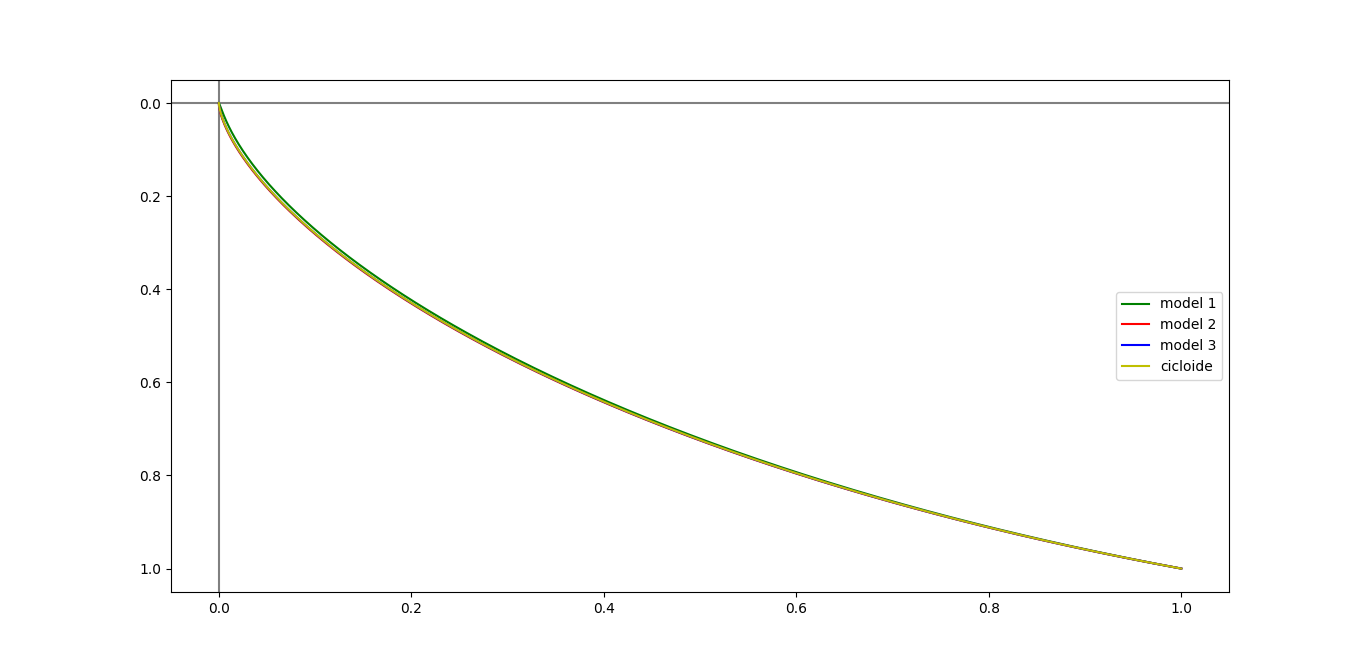
\includegraphics[width=0.7\textwidth]{Aprox_1_1.png}
            }
        \subfigure[Tram inicial]
            {
            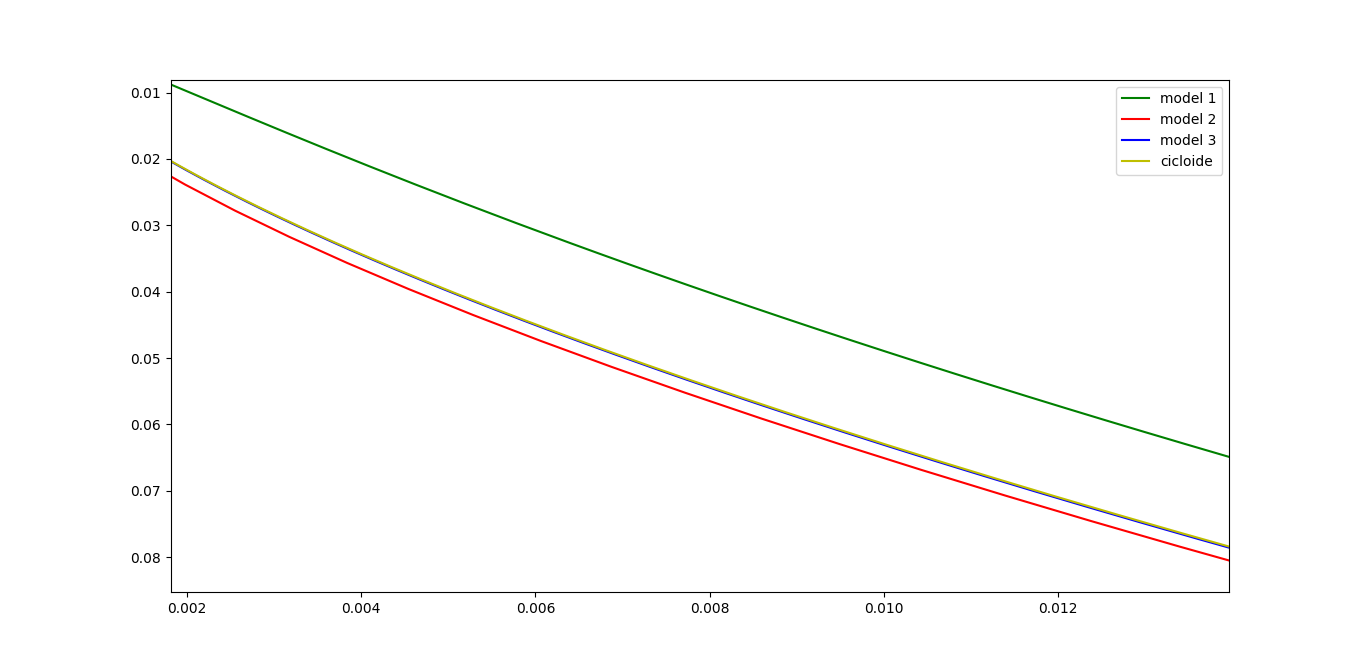
\includegraphics[width=0.45\textwidth]{Aprox_1_1_inici.png}
            }
        \subfigure[Tram final]
            {
            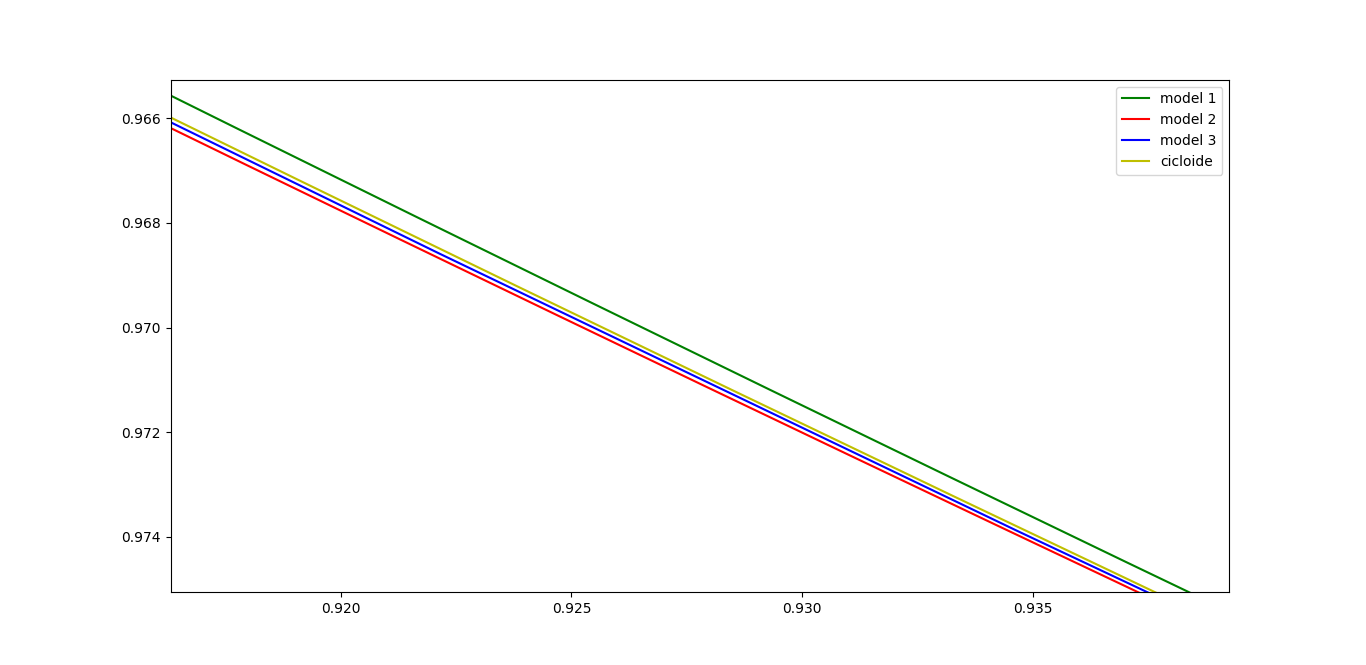
\includegraphics[width=0.45\textwidth]{Aprox_1_1_final.png}
            }
        \caption{Aproximació de la braquistòcrona per a n = 500, F = (1,1)}
        \label{Aprox_1_1}
    \end{center}
\end{figure}

\begin{figure}[H]
    \begin{center}
        \subfigure[Corba completa]
            {
            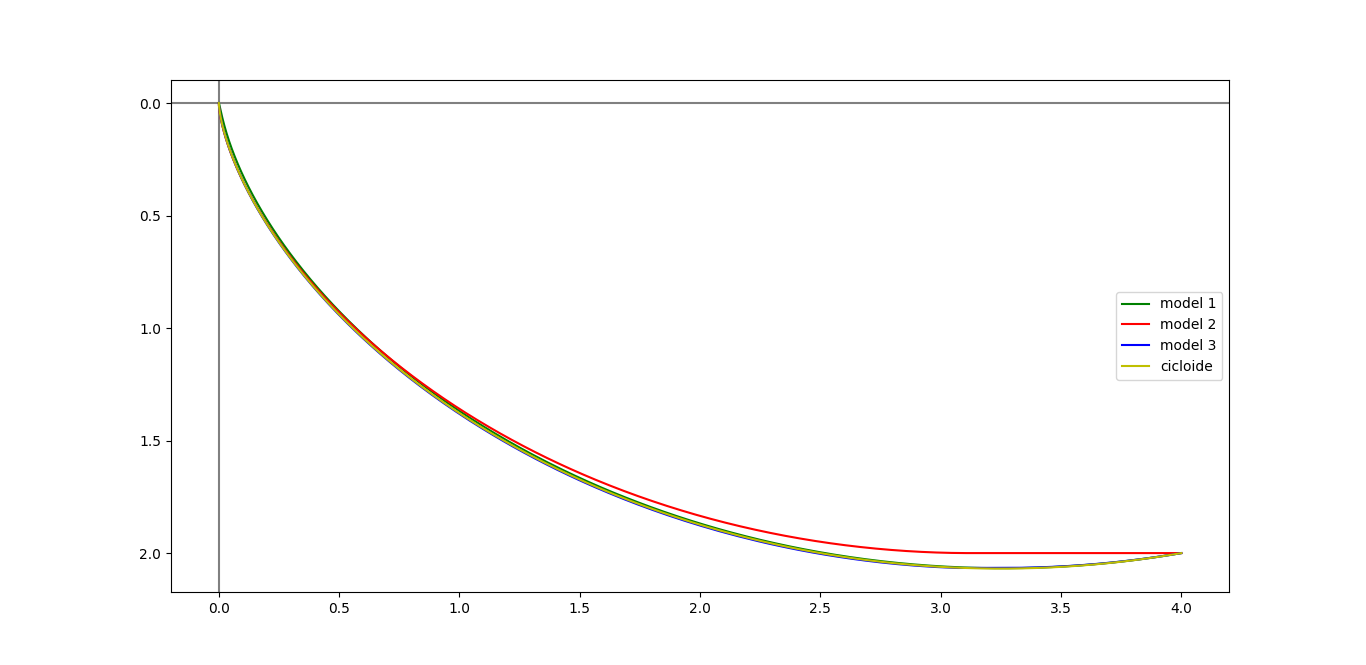
\includegraphics[width=0.7\textwidth]{Aprox_2_4.png}
            }
        \subfigure[Tram inicial]
            {
            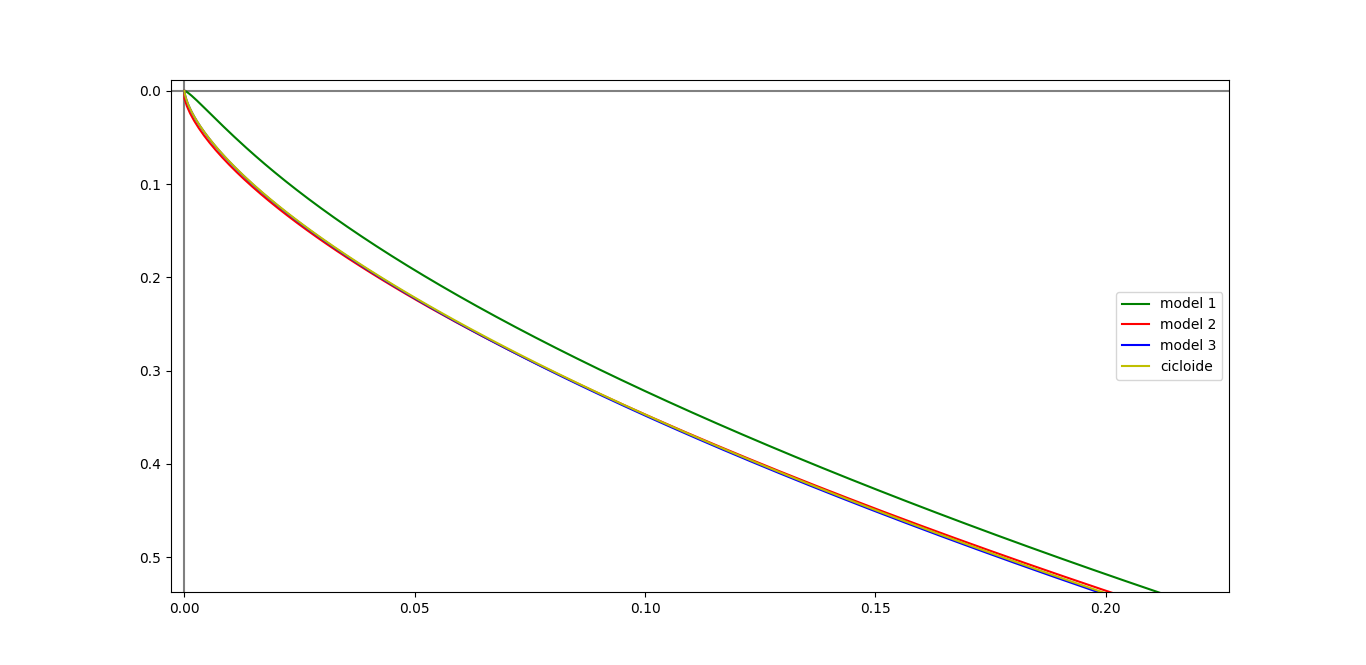
\includegraphics[width=0.45\textwidth]{Aprox_2_4_inici.png}
            }
        \subfigure[Tram final]
            {
            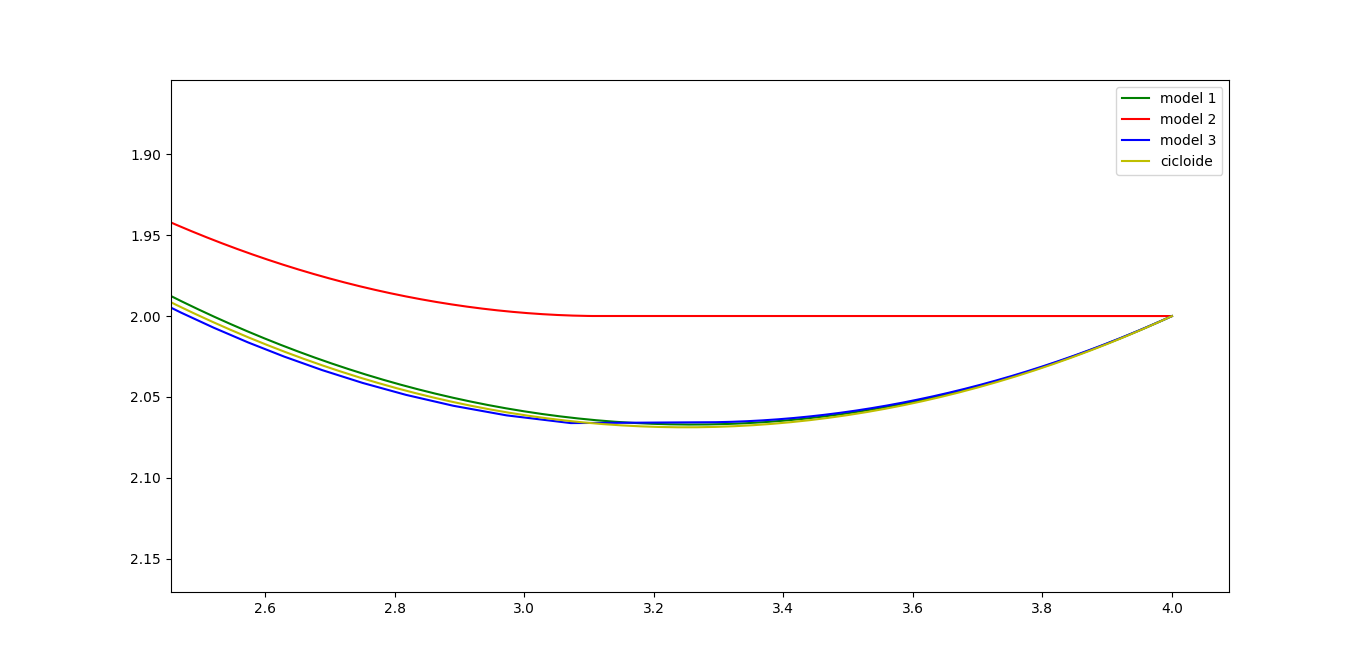
\includegraphics[width=0.45\textwidth]{Aprox_2_4_final.png}
            }
        \caption{Aproximació de la braquistòcrona per a n = 500, F = (4,2)}
        \label{Aprox_4_2}
    \end{center}
\end{figure}


\subsection{Implementació del primer model a AMPL}
\begin{lstlisting}
param n >= 0;
param a >= 0;
param b >= 0;
param g >= 0;
param eps >= 0;

param x{i in 0..n} = a*(i/n)^2;

var y{0..n} >= eps;

# Funcio objetiu
minimize velocitat:
		1/sqrt(2*g) * sum {i in 0..n-1} sqrt( ((x[i+1]-x[i])^2 + (y[i+1]-y[i])^2) / abs(y[i]) );

# Restriccions
subject to y_inicial:
	y[0] = eps;

subject to y_final:
	y[n] = b;
\end{lstlisting}

\subsection{Implementació del segon model a AMPL}
\begin{lstlisting}
param n >= 0;
param a >= 0;
param b >= 0;
param g >= 0;
param eps >= 0;

param y{i in 0..n} = b*(1-((n-i)/n)^2) + eps;

var x{0..n} >= 0;

# Funcio objetiu
minimize velocitat:
		1/sqrt(2*g) * sum {i in 0..n-1} sqrt( ((x[i+1]-x[i])^2 + (y[i+1]-y[i])^2) / abs(y[i]) );

# Restriccions
subject to x_inicial:
	x[0] = 0;

subject to x_final:
	x[n] = a;
\end{lstlisting}

\subsection{Implementació del tercer model a AMPL}
\begin{lstlisting}
param n >= 0;
param a >= 0;
param b >= 0;
param g >= 0;
param eps >= 0;

var x{i in 0..n} >= 0 default a*i/n;
var y{i in 0..n} >= eps;

# Funcio objetiu
minimize velocitat:
		1/sqrt(2*g) * sum {i in 0..n-1} sqrt( ((x[i+1]-x[i])^2 + (y[i+1]-y[i])^2) / abs(y[i]) );

# Restriccions
subject to x_inicial:
	x[0] = 0;

subject to x_final:
	x[n] = a;

subject to y_inicial:
	y[0] = eps;

subject to y_final:
	y[n] = b;
\end{lstlisting}

\section{Convexitat del segon model}
Vegem que el seguent problema és convex:
\begin{equation*}
    \left\{
    \begin{array}{ll}
        \displaystyle{\max\limits_{\substack{x_i \in \mathbb{R}_{\ge0} \\ \forall i = 0,1,\hdots,n}}} & \displaystyle{z = \frac{1}{\sqrt{2g}} \sum_{i = 0}^{n-1} \sqrt{\frac{(x_{i+1}-x_i)^2+(y_{i+1}-y_i)^2}{y_i}}} \\
        s.a.: & \displaystyle{x_0} = 0 \\
        & \displaystyle{x_n} = a \\
    \end{array}
    \right.
\end{equation*}

Un problema serà convex quant ho siguin tant la funció objectiu com la regió factible.

\subsection{Convexitat de la regió factible}
La regió factible està definida per constriccións lineals i, per tant, és convexa.

\subsection{Convexitat de la funció objectiu}
Sabem que la suma de funcións convexes i multiplicació d'un escalar positiu per una funció convexa són funcions convexes. Per tant, donat que $\frac{1}{\sqrt{2g}}$ és positiu, n'hi ha prou en comprovar que les seguents funcions són convexes:
$$f_i = \sqrt{\frac{(x_{i+1}-x_i)^2+(y_{i+1}-y_i)^2}{y_i}} \hspace{.25cm} \forall i = 0,1,\hdots,n-1$$

Donat que les $y$'s estan fixades tal que $y_i > 0 \hspace{.25cm} \forall i = 0,1,\hdots,n$ i $y_i < y_{i+1} \hspace{.25cm} \forall i = 0,1,\hdots,n-1$. Les funcions $f_i$ són $\mathcal{C}^2$, doncs són suma y composició de funcións que ho son. \vspace{.25cm}

A classe de teoria hem vist que:
$$f \in \mathcal{C}^2\text{ es convexa en } \Omega \subseteq \mathbb{R} \text{ convex i no buit } \Longleftrightarrow \nabla^2f \succcurlyeq 0 \text{ en } \Omega$$

La hessiana de les funcions $f_i$ és la seguent:
$$
\nabla^2 f_i = 
\begin{pmatrix}
    \frac{1}{\sqrt{y_i}} \frac{(y_{i+1} - y_i)^2}{((x_{i+1} - x_i)^2 + (y_{i+1} - y_i)^2)^{\sfrac{3}{2}}} & \frac{1}{\sqrt{y_i}} \frac{- (y_{i+1} - y_i)^2}{((x_{i+1} - x_i)^2 + (y_{i+1} - y_i)^2)^{\sfrac{3}{2}}} \\
    \frac{1}{\sqrt{y_i}} \frac{- (y_{i+1} - y_i)^2}{((x_{i+1} - x_i)^2 + (y_{i+1} - y_i)^2)^{\sfrac{3}{2}}} & \frac{1}{\sqrt{y_i}} \frac{(y_{i+1} - y_i)^2}{((x_{i+1} - x_i)^2 + (y_{i+1} - y_i)^2)^{\sfrac{3}{2}}}
\end{pmatrix}
$$

Podem veure que la hessiana de la funció és semidefinida positiva ja que els menors prinicipals són $\ge 0$ (les dos entrades de la diagonal principal són $> 0$, i el $det(\nabla^2f) = 0$). \vspace{.25cm}

Per tant, hem vist que $\{f_i\}_{i=0}^{n-1}$ són semidefinides positives, cosa que implica que $\{f_i\}_{i=0}^{n-1}$ són convexes i, per tant, z és convexa.

\section{Conclusions}
Hem modelitzat el problema de la braquistocrona de tres maneres diferents per a aproximar la corba amb una poligonal de $n+1$ punts. En tots els models l'aproximació és millor com més gran és la $n$ doncs augmentem el nombre de punts de la poligonal. \vspace{.25cm}

El primer model sempre genera una bona aproximació. Però en el tram inicial de la corba es troba una mica per sobre de la braquistocrona. \vspace{.25cm}

Per altre banda, hem vist que el segon model generarà una bona aproximació per a punts tal que $\frac{a}{b} \le \frac{\pi}{2}$. \\
Per a punts que no compleixen la condició, $f^{-1}$ (la funció que volem aproximar en aquest model) no està ben definida perquè $f$ no es injectiva, cosa que fa que no ens doni una bona aproximació de la corba tal com es pot observar en la Figura \ref{Aprox_4_2}. \\
En canvi, per a punts que compleixin la condició, com que el problema és convex, si trobem un punt estacionari qualsevol aquest serà òptim global. Per tant, tindrem la millor aproximació possible (per a $n$ i $y$'s fixades). \vspace{.25cm}

Per últim el tercer model ha generat una bona aproximació en els dos casos, però en aquest és molt important proporcionar uns valors inicials a les variables prou bons, per evitar minims locals. \\
Per exemple si inicialitzem les variables a zero o $\varepsilon$, tal com fa minos en els altres mètodes ens queden tots els punts a l'inici i la solució és una recta del punt $O$ a $F$. \\
Un altre exemple és si inicialitzes els punts $p_i = (x_i, y_i)$ en punts equidistants en el segment que uneix $O$ i $F$, el resultat dona un minim local, on la corba és la recta entre els punts $O$ i $F$.

\end{document}
